
\documentclass[foo.tex]{subfiles}
\begin{document}

\section{Galactic Chemical Evolution}
\label{sec:gce}

% fig 5
\begin{figure*}
\centering
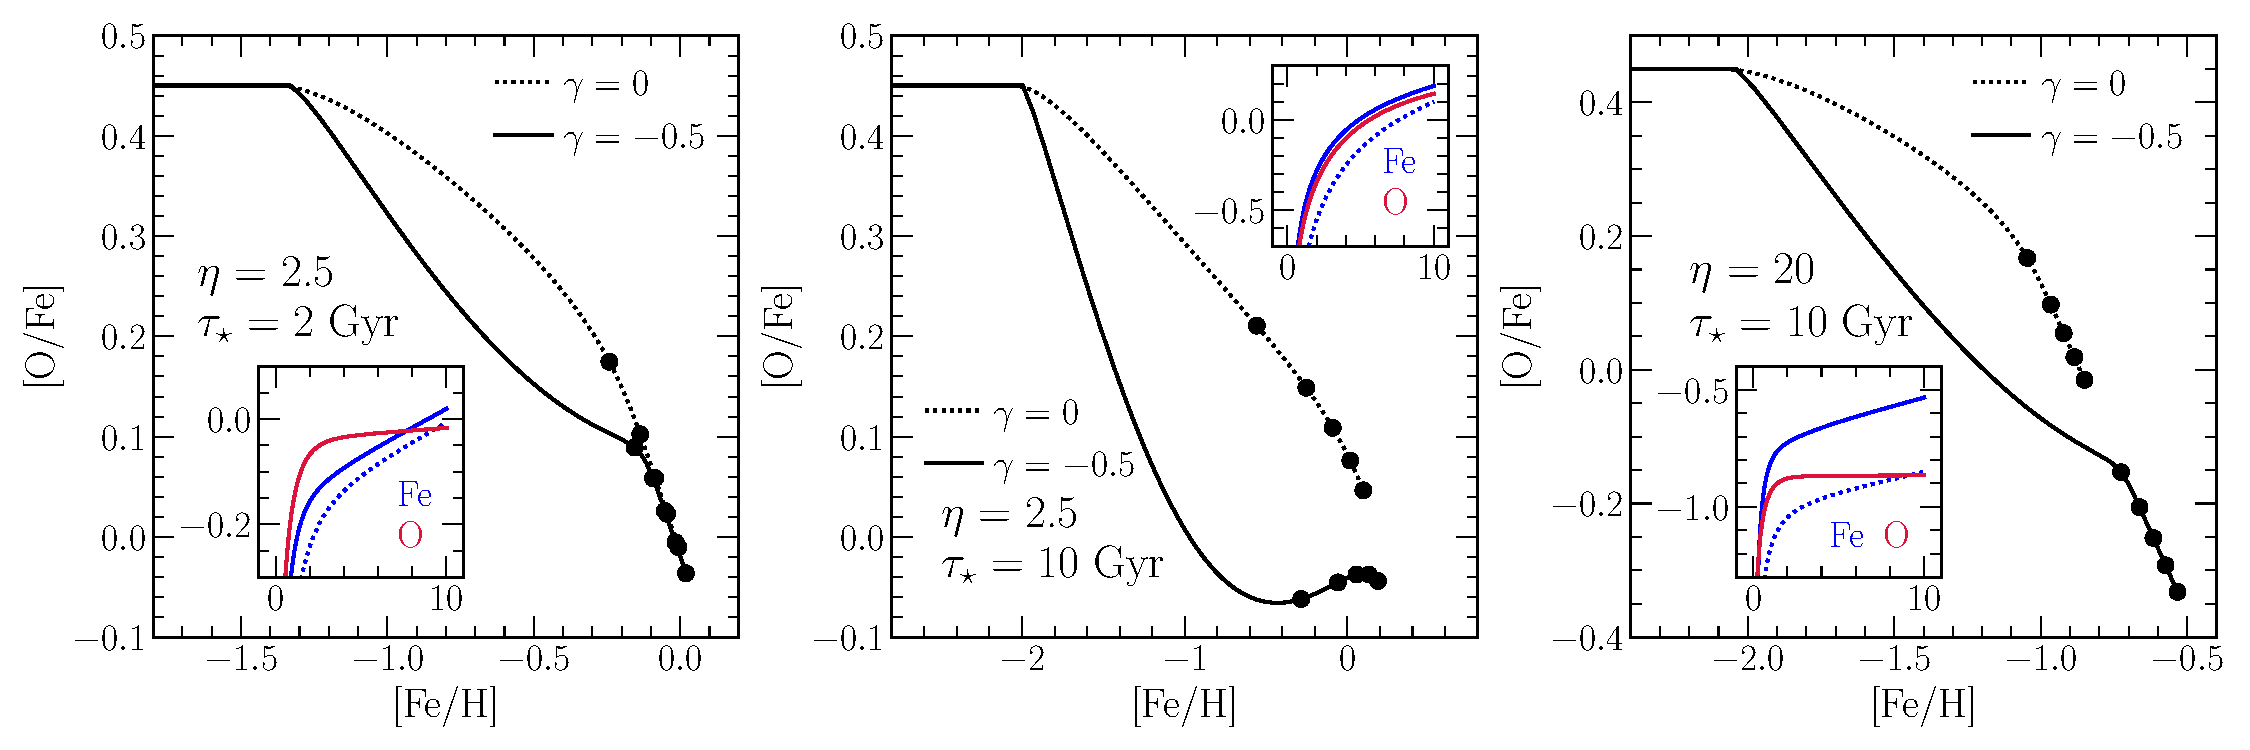
\includegraphics[scale = 0.46]{onezone_application.pdf}
\caption{
A comparison of one-zone galactic chemical evolution models based on
\citet[][for details, see their~\S~2]{Johnson2020} with ($\gamma = -0.5$,
solid) and without ($\gamma = 0$, dotted) metallicity-dependent SN Ia rates.
Tracks denote the O and Fe abundances in the interstellar medium parametrized
as a function of time with points marked at~$T = 2$, 4, 6, 8, and 10 Gyr.
Insets illustrate [O/H] and [Fe/H] as a function of time in Gyr for the
corresponding model.
We note on each panel the choice of the outflow mass-loading factor~$\eta$ and
the star formation efficiency timescale~$\tau_\star$.
}
\label{fig:onezone_app}
\end{figure*}

The realization that SN Ia rates likely depend on metallicity with a
$\gamma = -0.5$ dependence has important implications for galactic chemical
evolution models, which typically assume metallicity-independent rates.
To demonstrate this, we briefly explore several one-zone models based
on~\citet{Johnson2020} which predict the evolution of O (produced only in
massive stars) and Fe (produced in both massive stars and SNe Ia).
We use an exponential SFH with an e-folding timescale of~$\tau_\text{sfh} = 6$
Gyr and a minimum delay of~$t_\text{D} = 100$ Myr before the onset of SNe Ia
from a given stellar population.
For metallicity-dependent rates, we simply apply a~$(Z / Z_\odot)^{-0.5}$
prefactor to their Fe yield of~$y_\text{Fe}^\text{Ia} = 0.0017$, which assumes
that the shape of the DTD does not vary with metallicity -- only the
normalization.
Otherwise, these models are the same as~\citet{Johnson2020}.
\par
Fig.~\ref{fig:onezone_app} illustrates the predictions of this SFH with
$(\eta, \tau_\star) = (2.5, 2~\text{Gyr}), (2.5, 10~\text{Gyr})$, and
$(20, 10~\text{Gyr})$ where~$\eta \equiv \dot{M}_\text{out} / \dot{M}_\star$ is
the mass-loading factor describing the efficiency of outflows and
$\tau_\star \equiv M_\text{gas} / \dot{M}_\star$ is the inverse of the
star formation efficiency.
These values are appropriate for the Solar neighbourhood with efficient (left
panel) and inefficient (middle panel) star formation and for a dwarf galaxy
(right panel).
In all cases,~$\gamma = -0.5$ predicts a much more abrupt descent from the
high [O/Fe] plateau because of the higher Fe yield at low metallicity.
If incorporated into GCE models, this could impact the inferred evolutionary
timescales of the thick disc, known to host many of the high [O/Fe] stars in
the Milky Way~\citep{Hayden2017}.
When the equilibrium abundance is near-Solar but star formation is slow (middle
panel), the model predicts a ``secondary plateau'' in [O/Fe] because the Fe
enrichment rate slows down due to the metallicity-dependence of the yield
(see inset).
This is a noteworthy theoretical prediction because generally
[$\alpha$/Fe] and [Fe/H] reach equilibrium at similar times and no secondary
plateau arises~\citep[e.g.,][]{Weinberg2017}.
\par
These models are intended to be illustrative rather than quantitative.
In general, the only regions of chemical space where~$\gamma = 0$ and
$\gamma = -0.5$ agree are at near-Solar abundances and along the high [O/Fe]
plateau, which occurs before the onset of SN Ia enrichment.
A~$\gamma = -0.5$ scaling has the strongest impact at low~$Z$, where the
metallicity-dependence of the yield shifts the Fe abundances by~$\sim$0.5 dex
in this example.
% The considerable impact that a~$\gamma = -0.5$ scaling has on the predictions
% indicates that evolutionary parameters inferred from one-zone model fits to
% multi-element abundance ratios may need revised.
% A~$\gamma = -0.5$ scaling has the strongest impact for dwarf galaxies (right
% panel) where the metallicity-dependence of the yield shifts the Fe abundances
% by~$\sim$0.5 dex in this example.

\end{document}
